\chapter{Three Traits, Constructive Conflict, and the Growth of Trust}

This short interview does not proceed by blackboard derivation, but it does have a precise logical spine. We begin with a concrete hiring question, move immediately to a triad of desired traits, and then meet a paradox: the very people we most want to work with may still argue intensely. The speaker's answer is that this tension is not an exception to the rule. Under the right conditions, conflict is part of the mechanism by which a founding team discovers the best path forward and learns to trust one another.

\section{The Selection Question}

The opening question is crisp: what do we look for when we assemble a leadership team or hire people for a company? That framing matters. We are not yet discussing culture in the abstract, or leadership in the heroic sense. We are looking for a selection rule.

A compact way to hold the structure in mind is to introduce a purely editorial shorthand:
\begin{equation}
T = \{H,I,C\},
\end{equation}
where \(H\) denotes honesty, \(I\) intelligence, and \(C\) coachability, that is, the ability to take constructive feedback.

The notation is only a convenience. The interview itself gives us no weights, no score, and no ranking among the three items. The natural reading is conjunctive rather than additive: the speaker is naming three conditions that belong together.

\section{Honesty, Intelligence, and Coachability}

The answer arrives in a clipped rhythm. First, we are told to work with honest people. Then with intelligent people. Then with people who can take constructive feedback. The shortness of this list is one of the clip's strengths: the speaker is not giving a grand doctrine, but a practical filter.

\begin{definition}
For the purposes of these notes, we will call \(C\) the condition of coachability:
\begin{equation}
C \equiv \text{ability to take constructive feedback}.
\end{equation}
This is a compact reconstruction of the speaker's wording, not a formula stated in the interview.
\end{definition}

The next correction is crucial. The standard is not merely external. The speaker adds that this includes oneself. In that sense the third condition is reflexive:
\begin{equation}
C = C_{\text{self}} \wedge C_{\text{other}}.
\end{equation}
One must be able to receive correction from the same people one is evaluating.

We can summarize the three criteria as follows:
\begin{itemize}
\item \(H\): we need people whose statements and commitments can be trusted.
\item \(I\): we need people capable of understanding the problem and seeing consequences.
\item \(C\): we need people who can absorb criticism without the team collapsing into defensiveness.
\end{itemize}

The third term does more work than the first two. Honesty and intelligence are easy to name. Coachability begins to tell us how a team actually behaves once serious work starts.

\section{The First Tension}

At this point the clip makes its decisive turn. The list is clean, almost too clean, and the speaker immediately disturbs that neatness: even with the right people, we are not always going to get along.

\subsection{Question \& Answer}

\paragraph{Question.} If these are the right people to work with, why should there be so much friction among them?

\paragraph{Answer.} Because productive teams are not defined by the absence of disagreement. They are defined by the way disagreement is used. Honest, intelligent, coachable people are often precisely the people who can argue hardest about the path forward without treating the argument itself as a sign that the partnership is broken.

This is the conceptual hinge of the lecture. The first half names the initial conditions; the second half explains what those conditions make possible.

\section{Conflict as Search for the Best Path}

The speaker resolves the tension with a re-interpretation of conflict. Outsiders thought that the two founders were on the verge of destroying each other. The speaker says otherwise: what they were doing was fleshing out the best path forward, or the best idea forward. The disagreement was not noise around the work. It was part of the work.

\begin{definition}
We will call a disagreement \emph{constructive} when its operative aim is not personal victory but clarification of the best path forward.
\end{definition}

In a compact schematic form, the interview's causal chain can be written as
\begin{equation}
\text{constructive conflict}
\;\Rightarrow\;
\text{clearer best path}
\;\Rightarrow\;
\text{greater trust}
\;\Rightarrow\;
\text{more independent decisions}.
\end{equation}

This is not a law of management in any hard scientific sense. It is a disciplined summary of the mechanism the speaker is describing. The important point is that conflict is reclassified. Once it is directed toward the problem rather than toward ego, it becomes a search procedure.

\begin{figure}[h]
\centering
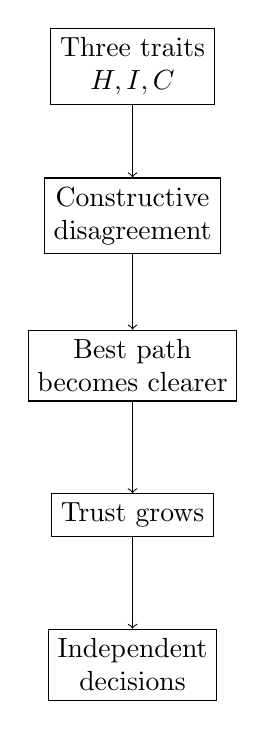
\begin{tikzpicture}
\node[draw, align=center] (traits) at (0,0) {Three traits\\\(H,I,C\)};
\node[draw, align=center] (conflict) at (0,-1.9) {Constructive\\disagreement};
\node[draw, align=center] (path) at (0,-3.8) {Best path\\becomes clearer};
\node[draw, align=center] (trust) at (0,-5.7) {Trust grows};
\node[draw, align=center] (indep) at (0,-7.6) {Independent\\decisions};
\draw[->] (traits) -- (conflict);
\draw[->] (conflict) -- (path);
\draw[->] (path) -- (trust);
\draw[->] (trust) -- (indep);
\end{tikzpicture}
\caption{Schematic reconstruction of the sequence described in the interview. The diagram is not taken from a board or slide; it simply makes the spoken logic visible.}
\end{figure}

\section{A Small but Revealing Example}

The concrete example is memorable because it is so ordinary. The founders had strong arguments over which shade of red to use on the first product packaging. This detail matters precisely because it is not a grand strategic crisis. The issue itself turned out to be inconsequential, but the process of arguing through it was not.

That is the point we should preserve. Teams do not build trust only by surviving existential moments. They also build trust by learning how to reason together in small, irritating, repetitive decisions where personality can easily overtake judgment. A dispute over packaging color is therefore not an irrelevant anecdote. It is a test case.

We can say the same thing more formally. Let the substantive importance of a decision be small, but let the style of argument be serious and honest. Then the informational value of the argument for the relationship may still be large. The lecture's emphasis falls not on the object being debated, but on what the debate reveals about the people involved.

\section{Trust and the Capacity for Independent Judgment}

The clip closes by describing the payoff of this process. Through repeated argument the founders became closer friends, trusted each other more, and came to allow each other more room for independent decisions. In other words, constructive conflict does not merely solve isolated problems. It changes the state of the partnership.

A cautious way to formalize the speaker's claim is to let \(\tau_n\) denote the level of mutual trust after the \(n\)-th serious disagreement. Then the narrative suggests the update rule
\begin{align}
\tau_{n+1} &= \tau_n + \Delta_n,\\
\Delta_n &> 0 \qquad \text{when the disagreement remains oriented toward the best path forward.}
\end{align}

Again, this is an editorial model, not a measured equation from the interview. But it captures the direction of the claim. The repeated episode is not merely endured; it is converted into trust.

We can make the logic explicit as a short derivation.
\begin{enumerate}
\item Begin with teammates selected for honesty, intelligence, and coachability.
\item Expose real decisions to open disagreement rather than suppressing conflict prematurely.
\item Keep the argument attached to the problem itself, so that criticism is informative rather than merely hostile.
\item Each successful episode of this kind adds to the stock of mutual trust, represented schematically by \(\Delta_n>0\).
\item As trust rises, the need for constant direct supervision falls, and independent decisions become possible.
\end{enumerate}

The speaker's final remark gives the interpretation of the whole sequence: the early phase of friction was necessary. One had to go through it in order to reach that level of confidence with each other. This last point prevents us from sentimentalizing harmony. The lecture is not saying that all conflict is good. It is saying that some conflict is the price of building a team that can later function with freedom and confidence.

\section{Summary}

The argument of the clip is compact but sharp. We begin with a triad of hiring criteria: honesty, intelligence, and coachability. We then discover that these traits do not eliminate conflict. Rather, they make a certain kind of conflict usable. When disagreement is aimed at finding the best path forward, it can deepen trust instead of corroding it. Even arguments over something as small as a shade of red can therefore matter, because they train the team in how to think together. The final lesson is not merely whom to hire, but what those hires must be able to endure and transform once the real work begins.